\cleartooddpage[\thispagestyle{empty}]
\chapter{Gamma Ray Reconstruction}



\section{Image Reconstruction}\label{subsec:imgrecon}

Pixels have their peak charge found.
Images are cleaned of extraneous pixels.
The time gradient is fit to each image.
Pixels participating in the image are identified.
From the time gradient, the dc (??) counts are integrated in a time window that moves with the time gradient of the shower.
Images are identified.

\section{Position Reconstruction}\label{subsec:posrecon}
Images have their disp calculated.
The major axis of mulitiple images are traced.
The intersection of the axes, weighted by their disps the angles between axes, can then determine their original position.

\subsection{Angular Reconstruction Neural Network}
At high elevations, shower images are often at large intesection angles, while at lower elevations the intersections the images are more parallel.
This means that when the reconstruction position is found by intersecting image axes, small changes in the image orientation can result in large movements in the reconstructed position.

To better handle these near-parallel image axes at low elevations, the reconstructed position can be determined from more parameters than just the weighted image axes intersection points.
From simulations, the distance between the center of the hillas shower image and the reconstructed position can be calculated, where the angular distance between the two is the 'disp' parameter\cite{Senturk:2011}, shown in figure \ref{fig:dispdiagram}.

\begin{figure}[h]
  \begin{center}
    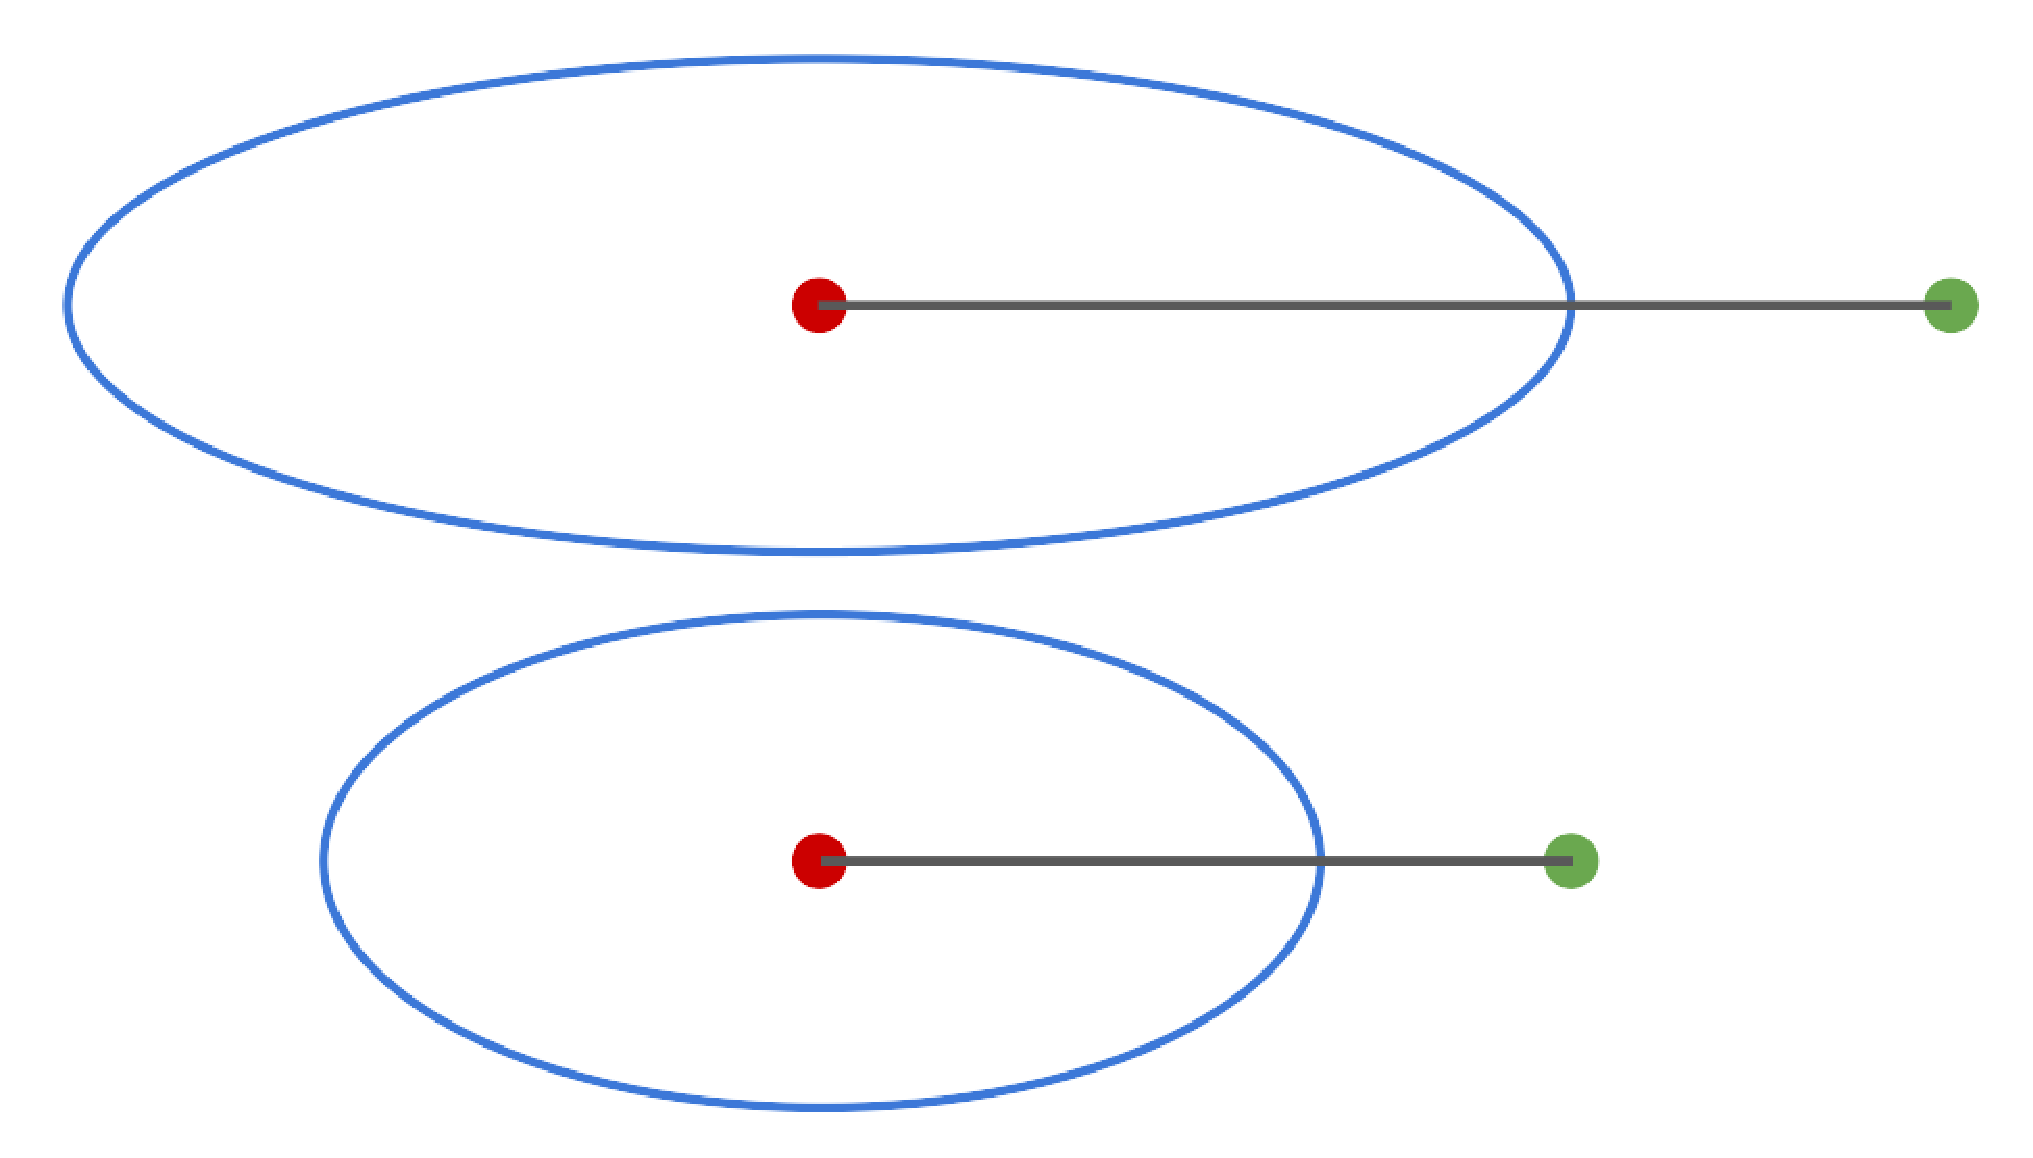
\includegraphics[width=0.5\textwidth]{images/thesis.dispdiagram.eps}
    \caption[Angular Reconstruction Disp]{The disp parameter is the angular distance between the center (red dot) of a hillas image (blue oval) and the true sky position (green dot).  Generally, longer shower images have a larger disp angle.}\label{fig:dispdiagram}
  \end{center}
\end{figure}

% https://veritas.sao.arizona.edu/wiki/index.php/BDT_Angular_reconstruction
The disp and other parameters for thousands of simulated showers can then be used to train a neural network that calculates the most probable disp for a given shower.
This most probable disp can then be used with the image axes intersection points to more accurately reconstruct the original gamma-ray point of origin.

Once the training is complete, it is tested on a separate set of 17,000 simulated events, which are plotted in figure \ref{fig:disptraining}.
The x axis describes the true disp value for each event, while the y axis describes the disp value predicted by the Boosted Decision Tree network, with a black line for the x=y line.
As the majority of the events fall on the line, we can conclude that the BDTs are able to predict the correct disp value for most images.

% made from screenshot of last slide in Dropbox/Presentations/20160719_Group_Meeting.key
\begin{figure}[h]
  \begin{center}
    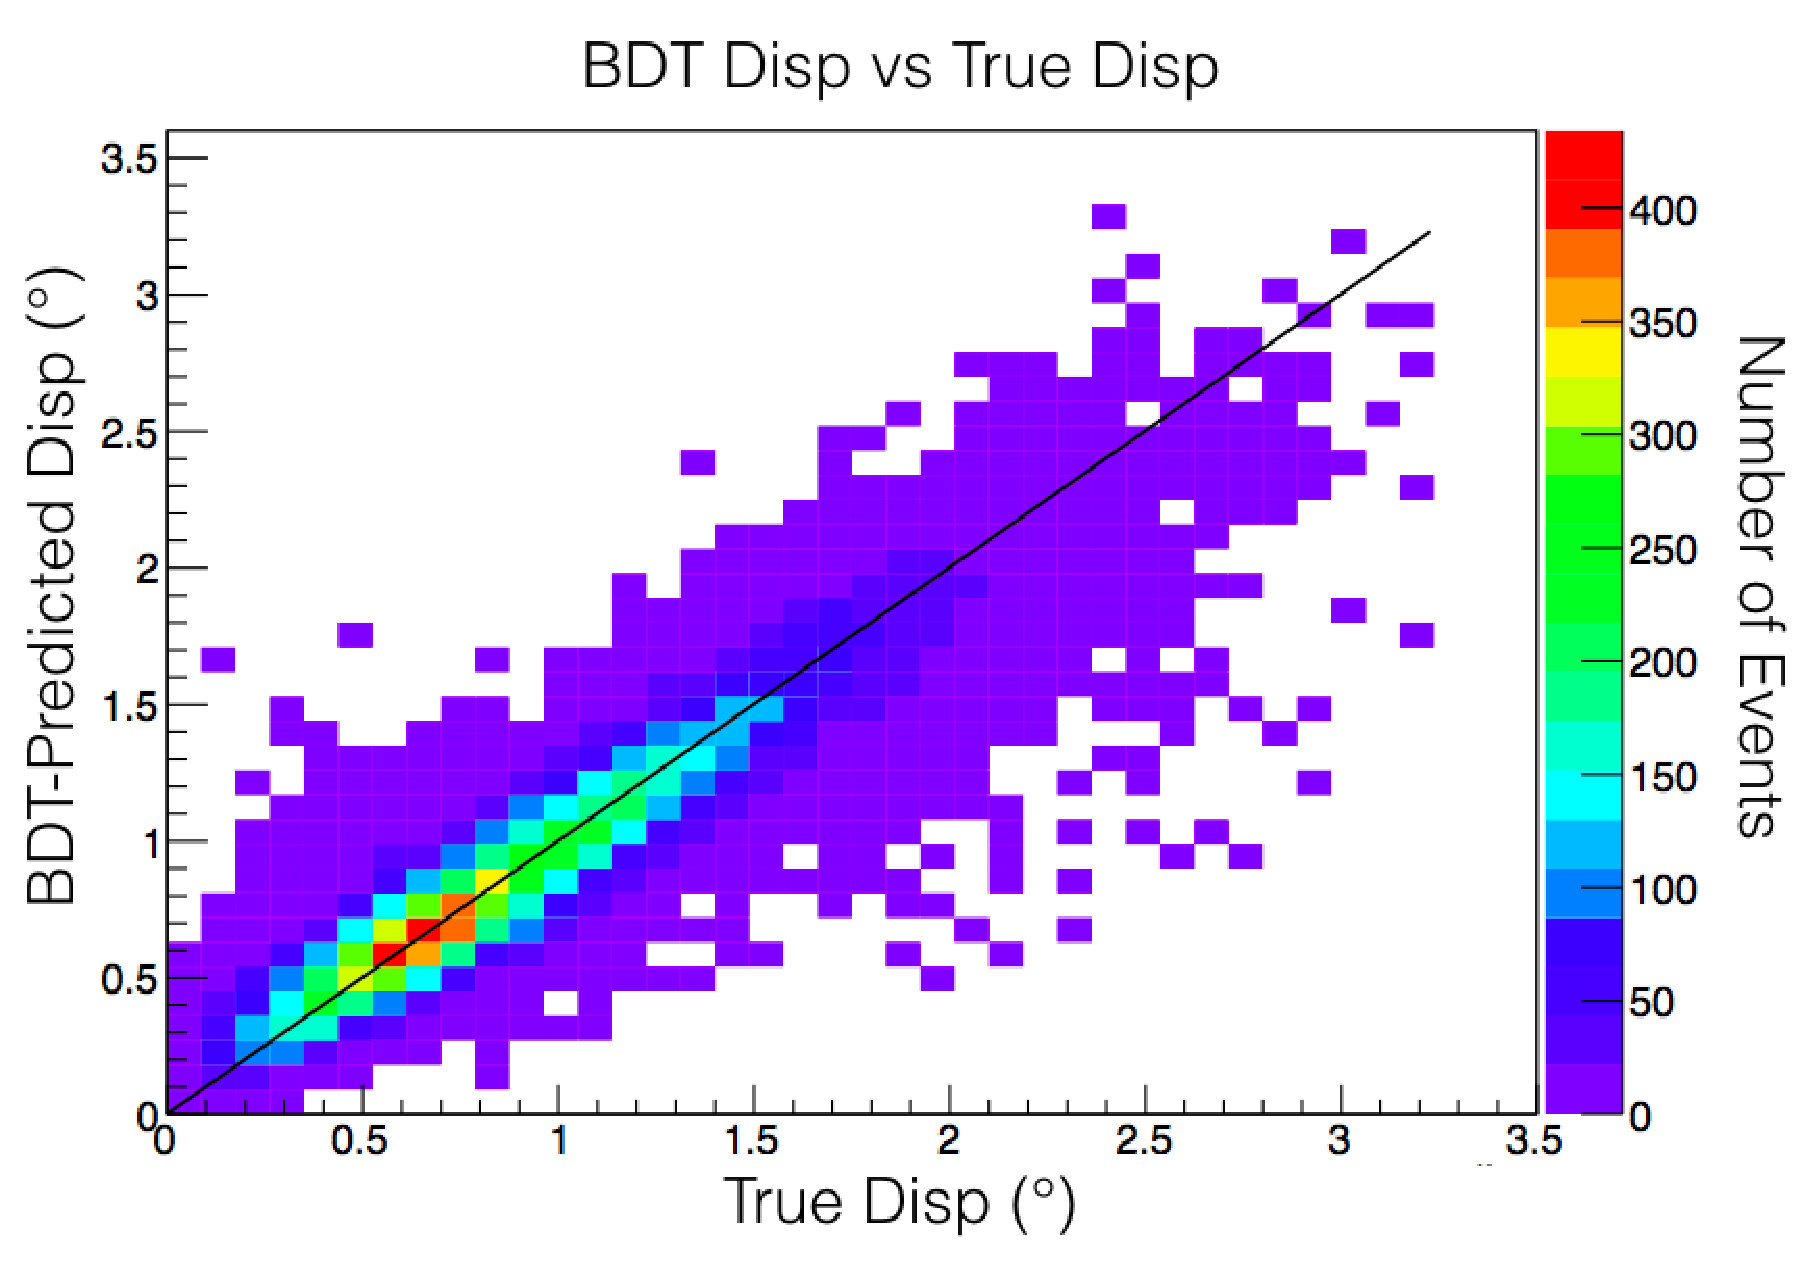
\includegraphics[width=0.85\textwidth]{images/disp_training.eps}
    \caption[Disp BDT Training]{The true disp vs the BDT-predicted disp, for \nicetilde17,000 gamma-ray event images in T1, from 500GeV to 200TeV.}\label{fig:disptraining}
  \end{center}
\end{figure}

Improved angular resolution plot??

\section{Energy Reconstruction}\label{subsec:enrecon}
A library of different showers is built, from a variety of elevations, energies, and distances from the camera.
This library can then be used to look up a real shower, find the most similar in elevation, shape, etc, and then reading that shower's library energy.


\section{Sensitivity}
% plot vs energy
Sensitivity is a measure of how difficult it is to get a signifiant detection.
It is often quantified by using simulations to predict the amount of observation time required to detect a simulated source at a given significance level.


\section{Effective Area}
% plot of effective area vs energy
Effective area is the measure of how many gamma rays a telescope can detect.
It is referred to as 'Effective' because the detection efficiency is not 100\% at all energies or all parts of the camera.
Instead it is 'effectivly' how large a detection area a telescope has, if it had perfect detection efficiency.
Different telescopes can use this number to compare roughly how many gamma rays can be detected in a given span of time.


\section{Energy Resolution}
% plot of energy resolution
Gamma rays and protons of different energies can produce similar-looking air showers.
Due to this, the reconstruction software cannot perfectly reconstruct gamma rays, which introduces errors into the different qualities of the gamma rays.
This means that when a gamma ray is reconstructed, it has a chance to be reconstructed at a lower or higher energy.
The consequence of this is that gamma rays of a given reconstructed energy can come from a distribution of true simulated energies.
Typically, simulations are run across a number of energies, and an 2D matrix is assembled, where one axis is the true simulated energy, and the other axis is bins of reconstructed energy.


\section{Point Spread Function}\label{sec:psf}
% plot of psf
In addition to the energy being slightly mis-reconstructed, the source position of the gamma ray can also be misreconstructed.
For a gamma ray telescope, a simple measure of this misreconstruction is to simulate many gamma rays at a single point in the sky, and look at how their reconstructed positions are distributed around that point.
This distribution is referred to as the Point Spread Function.
To first order, most current-generation point spread functions are gaussian distributions.


\section{Energy Dispersion}
Much like the point spread function in section \ref{sec:psf}, the energy reconstruction process is also imperfect.
This means that a gamma ray with a reconstructed energy could come from a distribution of true energies.
This can also be phrased that a group of gamma-rays with the same initial energy will have a distribution of reconstructed energies.
These distributions primarily are due to inherent randomness in the showers themselves.


\section{Energy Sensitivity and Zenith Angle}
% plot of energy sensitivity at 20zen and 65zen

As the telescope points at a lower elevation, the atmospheric volume that can be used to detect air showers greatly increases, leading to an increase in the telescope's effective areafor high energy showers.
The downside is that fewer low-energy gamma rays reach the volume of atmosphere being observed, 


\section{Comparison with Other Observatories}

% sensitivity comparison plots

CTA, HESS, Magic, HAWC, Fermi

\section{FITS Conversion for Gammalib and CTOOLs}

Once gamma rays have been reconstructed with event display, they must be converted to a FITS file format compatible with gammalib.
This format consists of a FITS file with an event list table, containing each gamma ray, its energy, position, and time.
This also includes meta information about the event list like the telescope's pointing target and the start and end times of the event list.
This FITS file can then be read into Gammalib and CTOOLS (cite??).

In addition to the event list, the instrument response functions (IRFs) must also be imported into Gammalib and Ctools.
These include effective areas, point spread funciton, energy dispersion, and background shapes for several dimensions in the IRF parameter space (energy, offset from camera center, telescope elevation/azimuth, noise, etc).
By default, all IRFs are stored in a single database, and each event list contains a reference to which part of the parameter space should be used with it.

However, the galactic center is at an elevation of 30\degree, much lower than most VERITAS observation targets.
At this elevation, with its field of view of 3.5\degree, the air mass column density ($g/cm^{2}$) is 20\% higher at the bottom of the camera than at the top.
Add to this that during a single 30 minute observation, the elevation of the Galactic Center can change by several degrees, means the airmass in view of the camera may change rapidly, meaning the IRFs may become time dependent.

To allow for this time dependence in the analysis, an alternate way of storing the IRFs was chosen, diagrammed in figure \ref{fig:fits_scheme}.
First, one observation (typically 20-30 minutes long) is broken up into \nicetilde3 minute chunks.
Each chunk is then converted to an event list, and saved to a FITS file.
In addition, the needed Effective Area, PSF, and background tables are also written to the same FITS file.
As each event list covers a small region in time, the IRF tables only need to contain the dimensions of the parameter space that can change during one chunk, such as event energy and distance from camera center.

\begin{figure}[h]
  \begin{center}
    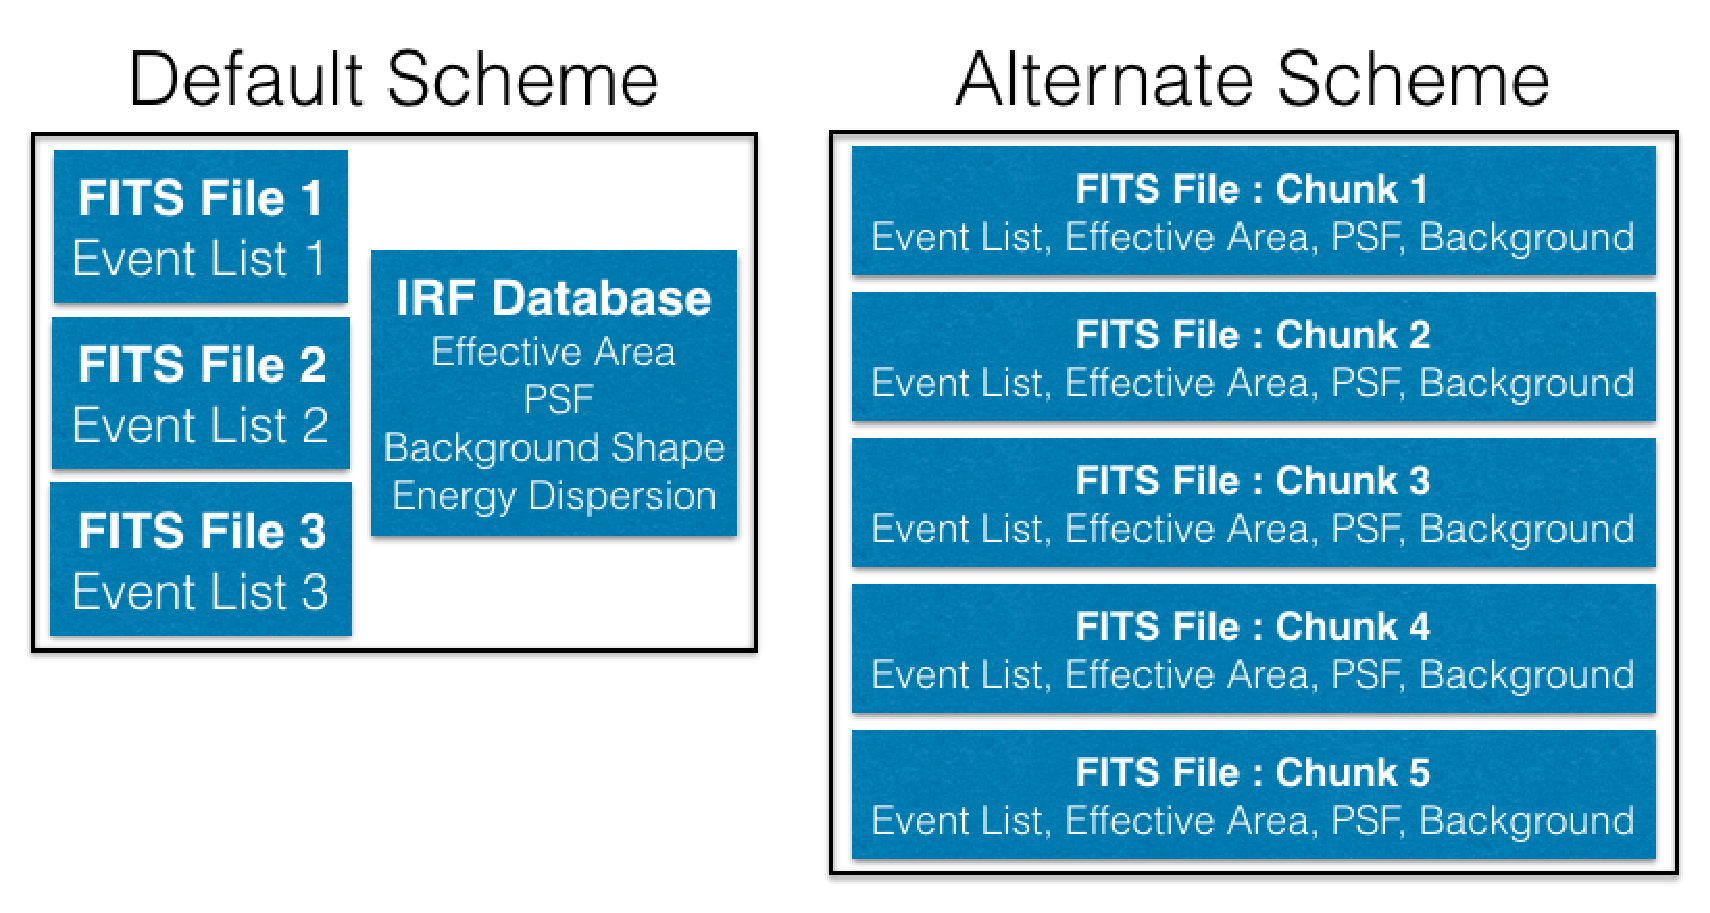
\includegraphics[width=0.75\textwidth]{images/FITS_diagrams.alternate_scheme.eps}
    \caption[FITS File Event Storage Schemes]{}\label{fig:fits_scheme}
  \end{center}
\end{figure}

The end result is that a 30 minute observation can be broken into \nicetilde10 FITS files (called chunks), where each chunk file is independent of any outside references, contains all IRF needed information, and only takes up \nicetilde100s KB.
This makes it ideal for an analysis program to automatically download any needed data over an internet connection, as each chunk is tiny and has no outside dependencies.
As gammalib and CTOOLS expect the default FITS file scheme, a python function was written to automatically load all event and irf tables from a single fits file, and import this information into gammalib's GObservation class.

There were minor issues with converting the IRFs that are noted in the following sections.

\subsection{PSF Fitting}

For the PSF, converting from Event Display to Gammalib has some issues.
Specifically, Gammalib tables store the PSF as the fit parameters of a King function (cite??).
A king function tends to fit gamma ray telescope PSF's better, due to its long tail (compared to a gaussian).
As the PSF in event display is stored as a histogram, with the number of events at each radial distance, it becomes necessary to fit a king function.
For roughly half of the parameter space, the king function fitter was unable to get a good fit (??).
When this happens, a default value of 0\degree is used as the PSF.


\subsection{Background Templates}

To produce a background, events are binned in camera coordinates and energy, and each bin is divided by the size of the bin's exposure in time, energy, and solid angle.
This allows for the likelihood engine to model the expected camera background of cosmic-ray events that pass all gamma-like cuts.
As the likelihood engine will apply a scale value to the background as part of its fitting, the background's absolute values matter much less than its relative values.

During the production of the initial low elevation background, some new effects were noted.
First a series of gamma-like events were taken from observations with no known gamma-ray sources.
These events are then divided into equal-statistics bins.
For each equal-statistic energy bin, all the contained events are binned in camera X and Y.

For a set of high-elevation observations, these backgrounds are shown in figure \ref{fig:back_highelev}.
It can be seen that all events are divided up into 3 equal-statistics energy bins in figure \ref{fig:back_highelev}.A.
Each energy bin is then binned in camera X and Y in figure \ref{fig:back_highelev}.B, .C, and .D.
It can be seen that at these high elevations, each energy bin is radially symmetric about the camera center.
This happens because gamma ray's point of origin and its shower image in the camera are usually several tenths of a degree away from each other.

\begin{figure}[h]
  \begin{center}
    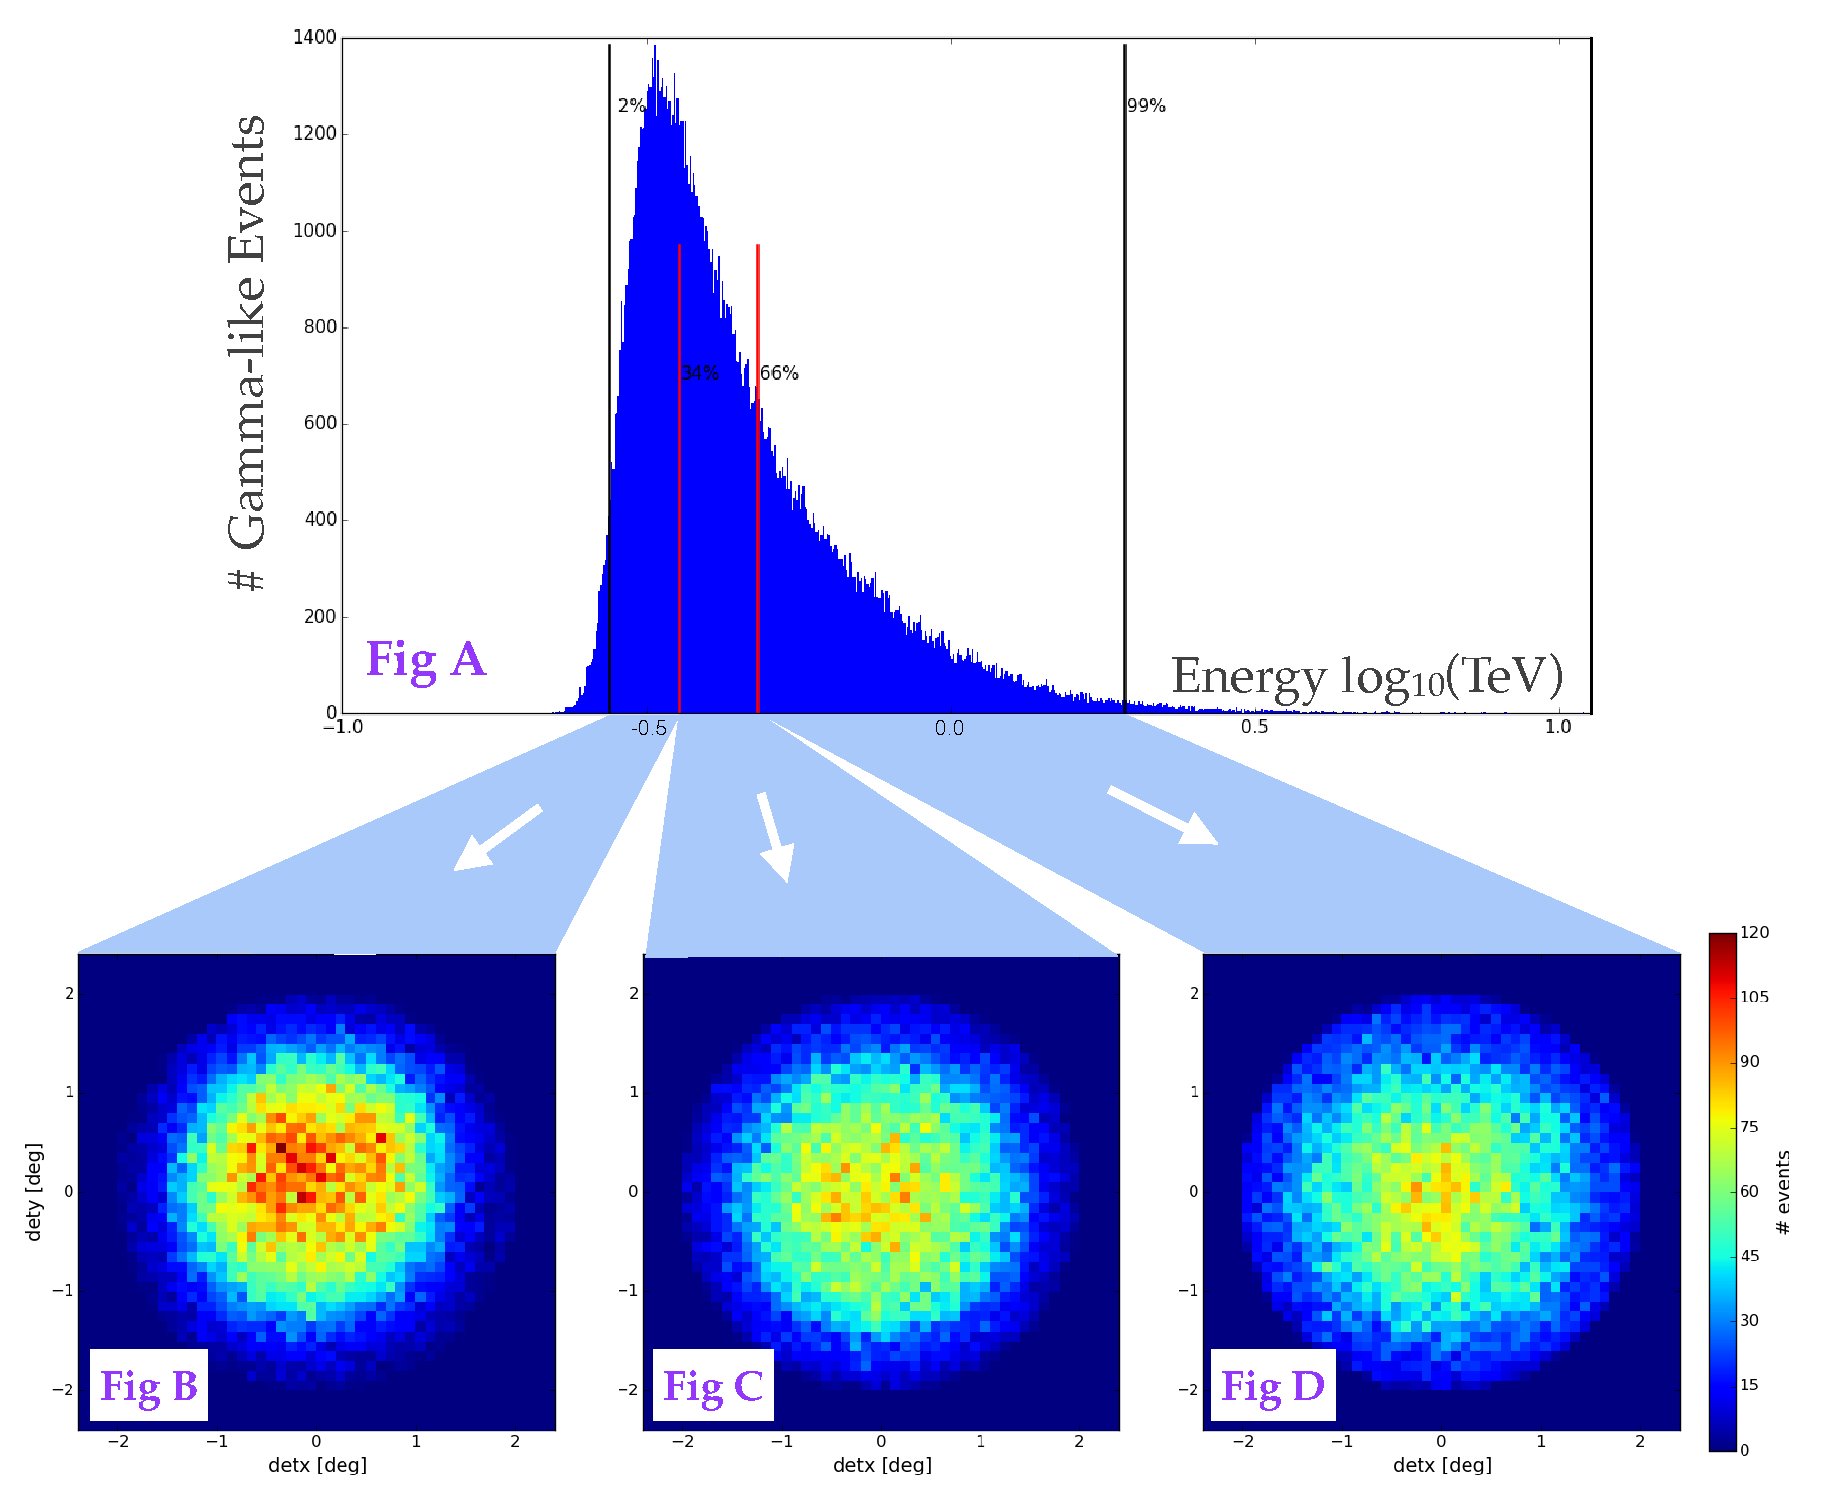
\includegraphics[width=\textwidth]{images/ctools/backgrounds.highelev.eps}
    \caption[FITS Background at High Elevations]{Gamma-like Events from 52 observations(livetime??) of M82 (in what elevation range??).  Events in Figure A are divided into 3 equal-statistics energy bins, and binned in Camera Coordinates in Figures B, C, and D.}\label{fig:back_highelev}
  \end{center}
\end{figure}


In figure \ref{fig:back_lowelev}, the same plots are constructed for a set of low-elevation (~28\degree) observations, using Galactic Center Off observations.
These are again divided in to equal-statistic energy bins, and then each energy bin is binned in camera coordinates.
It can be seen that in different energy bins, the background possesses different shapes.

\begin{figure}[h]
  \begin{center}
    \includegraphics[width=\textwidth]{images/ctools/backgrounds.lowelev29.eps}
    \caption[CTOOLS Background at \nicetilde29\degree Elevation]{15(livetime??) Sagittarius A* Off runs, between elevations 27.5\degree and 30\degree.  Events are divided into 6 equal-statistics energy bins, of which four are binned in Camera Coordinates in figures B, C, D, and E.}\label{fig:back_lowelev29}
  \end{center}
\end{figure}

\begin{figure}[h]
  \begin{center}
    \includegraphics[width=\textwidth]{images/ctools/backgrounds.lowelev26.eps}
    \caption[CTOOLS Background at \nicetilde26\degree Elevation]{10(livetime??) Sagittarius A* Off runs, between elevations 24\degree and 27.5\degree.}\label{fig:back_lowelev29}
  \end{center}
\end{figure}
















